\documentclass[UTF8]{ctexart}
\usepackage{xeCJK}
\author{Richard Gendal Brown, James Carlyle, Ian Grigg, Mike Hearn}
\date{2016年8月}
\title{Corda分布式账本平台:简介}
%%\setlength{\parskip}{\baselineskip}
\usepackage{amsfonts}
\usepackage{listings}
\usepackage{color}
\usepackage{epigraph}
\usepackage{graphicx}
\graphicspath{ {images/} }
\usepackage[export]{adjustbox}
\usepackage{float}
\usepackage{hyperref}
\usepackage[super,comma,sort&compress]{natbib}
\usepackage[nottoc]{tocbibind}
%\usepackage[natbibapa]{apacite}
\renewcommand{\thefootnote}{\alph{footnote}}
%\epigraphfontsize{\small\itshape}
\setlength\epigraphwidth{4.5cm}
\setlength\epigraphrule{0pt}
\begin{document}
\maketitle 
\begin{abstract}
由相互不信任节点组成的分布式账本可提供一个全局性单一数据库,用于存储机构与个人之间交易和债务的状态。目前为了保持各个独立账本之间数据同步,需要大量耗时的人工工作,而分布式账本可淘汰其中很大一部分。这也将提高金融业内现行的代码共享水平,以降低大众使用金融服务的成本。本公司推出Corda——一个为了实现以上目标而设计的平台。本文为一般读者提供高水平的介绍,而即将发布的技术白皮书会详细阐述Corda的设计理念与基础框架。
\end{abstract}
\newpage
\tableofcontents
\newpage
\section{引言}
我们R3坚信,分布式账本技术有潜力为金融服务行业带来变革,使业内客户与相关公司获益。我们的愿景是:未来金融协议将得到准确的存储与自动管理,每个人都能无误无缝地处理任何契约或合约。我们相信未来市场趋势将是:参与方达成的金融合约一旦被记录,就可以被准确无误地持有和共享。重复、调账、匹配失败和数据损坏都将成为历史。以资产为代表的孤岛将不再出现。

我们期望依赖已经被证明的技术,在现有的法律框架内,为金融服务场景创建一个共享账本架构。我们的理念可分为以下三类:满足机构的工程需要、关注非功能性的需求、可扩展性。

本文介绍了Corda平台的设计特点,我们相信这个平台对金融机构会是非常不错的选择。\footnote{读者可通过邮件联系作者:Richard Gendal Brown \href{mailto:richard@r3cev.com}{(richard@r3cev.com)}, James Carlyle \href{mailto:james@r3.com}{(james@r3.com)}, Ian Grigg \href{mailto:iang@r3.com}{(iang@r3.com)}, Mike Hearn \href{mailto:mike@r3.com}{(mike@r3.com)}}

\section{背景}
银行业敢于突破传统思维,较早地利用信息技术,将手工处理精确地自动化,将物理处理精确地数字化。然而,我们仍有机会改善这些新兴架构的成本与效率。 

值得一提的是,每个金融机构都以自己的角度维护着记录客户群和交易对方协议、地位的账本。同样,交易对方也以自己的角度维护着这样一个账本。这种重复会导致记录的不一致,需要交易各方耗费高昂成本来进行对账、调账和纠错。对同一笔交易,双方认知存在差异也是一个风险,并且可能是系统性风险。

多个金融机构的存在会促进竞争,多个技术平台的存在则会增加复杂性,产生运营风险。然而一直以来,这些风险不可避免,除非采用集中化的市场基础设施。由此看来,仅仅依靠合作公司提高技术而不提高自己的水平是行不通的。

集中化市场基础设施在提高机构间数据与商业逻辑共享度方面已有成效,但整体上看,金融交易领域的整合水平仍然远远低于网络时代的信息交换水平。

我们相信加密技术的进步,例如通常说到的区块链技术,提供了一个新的机遇:机构间安全共享记录的权威性系统。通过建立一个记录金融交易、处理商业逻辑的全新共享平台——一个可记录企业间所有协议的、权威性的全局性逻辑账本,为金融机构间(特别是但不限于交易后服务)的经济活动带来变革。这个架构会为金融行业带来一个全新的共享平台,这个平台之上的新老参与者及第三方都能展开竞争,竞相提供创新产品和服务。 

\begin{figure}[H]
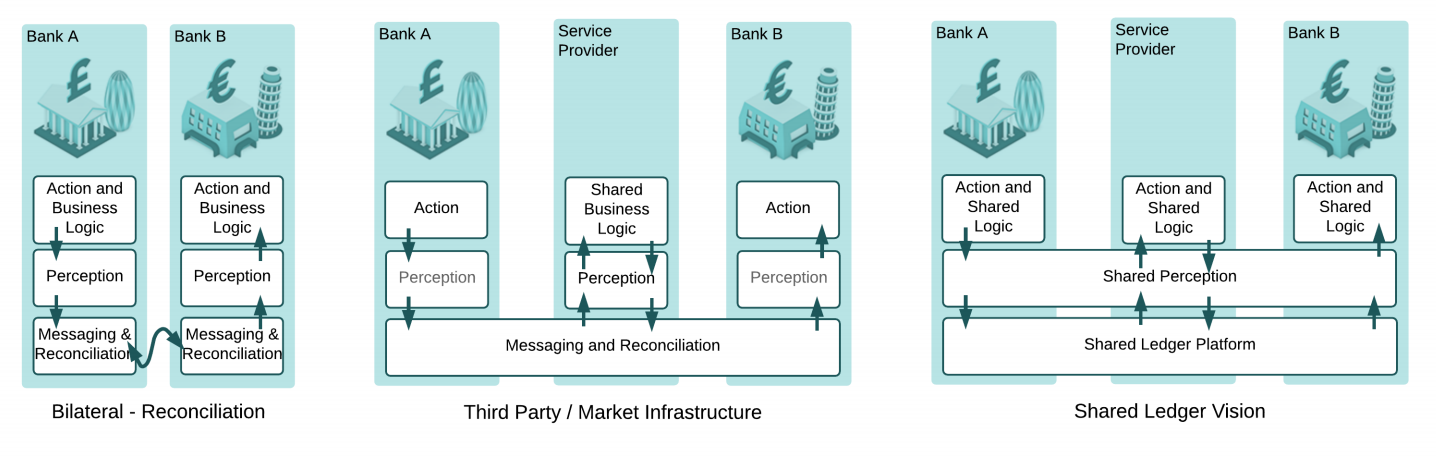
\includegraphics[scale=.5, center]{sharedlogic} 
\caption{上图所示,我们展示了三种状态的变化过程。第一种是参与方各自记录并管理自己的账本,处理所引发的不一致性和重复问题(\textit{``双边-协商"}),第二种是参与方将关键处理过程的权责委托给集中化服务商(\textit{``第三方/市场基础设施"}),进化到第三种,则是各方在开放性与竞争性基础上,使用新老服务提供商及市场基础设施提供者的服	务,合作维护一个共享账本,保证各方记录的一致性。}
\end{figure}


我们相信,更高质量的数据、更少的差异和更快的企业达成协议速度,将带来成本的大幅节约。而且,各个企业若使用这个共同架构,会形成一个新的平台让新老金融服务商展开竞争,更好地服务客户需求.未来,这样的平台也有可能在企业内部应用,现在企业内部用多个系统记录同笔交易,也是造成成本上升、操作复杂的一个主要原因。

\section{愿景}
长期来看,我们可以预想借助``全局性逻辑账本”,使所有经济活动参与者充分互动,任何参与方均可通过一种安全、一致、可靠、私密、权威的方式,来记录和管理彼此之间的协议。之所以称之为全局,是因为呈现给每个人的数据都是一样的;之所以符合逻辑,是因为其物理方式的实现会有所差异。最终可能形成的状态,将会是企业内部维护的权威账本系统被淘汰,由企业间可共享的全局性权威记录系统取而代之。 

\subsection{终态原则}
如果使用分布式账本技术,终态原则包括:
\begin{itemize}
	\item 账本上记录的事实无论在任何争议场合,都可被各方看作具有法律约束力的可用证据。
	\item 记录在账本上的事实是具有权威性的,而非存储在别处的权威数据的”影子“,因此直接通过平台便可达成决定。
	\item 参与方一旦达成协议,账本上的记录就是最终且不可变的。纠错或解约唯有通过后续交易来实现。这将促使公司不得不通过改进内部工作流程来提高准确度和质量标准。
	\item 原则上,任何授权参与方都可以直接访问账本,并通过账本来记录与交易对方达成的协议。任何参与方都不用被迫与其他方打交道,但是分级或等级制的市场模型可能会越来越少。 
	\item 通过提倡开放式的标准和私密性的访问,新老金融服务提供商都可以实现互联,展开竞争,提供差异化的服务,从而利于客户自由选择,促进业内竞争。
	\item 唯一能访问金融交易内容的是参与方本人,和其他具有合法知情权的人。
\end{itemize}

然而,这个愿景的最终实现需要过渡状态,比如最初只关注共享商业逻辑的参与方。现有的系统在可预见的未来将会一直存在,意识到这一点,在设计解决方案的时候就需要把现有系统的共存、整合与移植作为一个基础。这些过渡状态也可带来可观的价值,同时长期愿景的法律和其它非技术性问题也可着手解决。

需要强调的是,我们的远期目标是实现一个全局性逻辑账本,但是最后实现的可能是多种形式的分类账本。也许最后的情况是一种资产类别对应一个账本,账本的匹配具备自主性和灵活性,又保证不同商业服务间功能上和操作上的独立性。 

支撑这个愿景的架构和战略选择包括:
\begin{itemize} 
\item 只有对其管理的资产与协议有法定权益的人员能够访问此系统管理的记录。
\item 此系统管理的协议的变动将由计算机代码描述,这段代码必须获得相应法律文件的合法授权。
\item 为了确定如何处理合约失败问题,此系统提供了对合约代码升级的支持,以及关于争议解决流程的明确参考。这是因为就算在自动设定下,技术和人为因素也会导致出现合约争议情况。 
\item 成本、风险和监管负担(包括资本、流动资金和运营债务)的降低,创新产品和服务的出现,就意味着我们的愿景得到了成功实现。
\item 为了实现整个金融界的广泛应用,本系统的一部分必须且将会保持开放:开放源码、开放研发,开放标准。
\item 虽然此愿景使用到了诸如一个”平台“或”系统“的词语,我们认为实际设计仍是多层级的,可能由多个技术提供商竞争或合作提供不同组成部分。读者不应该想象我们把这个系统设计成了一个完全统一垂直整合的模式。
\item 此愿景还意味着,产品高层级所包含的知识产权可由参与建设的企业或组织持有。
\item 基于日益严重的网络犯罪和严峻的网络安全形式,本系统会采用高标准的安全设计来应对。
\end{itemize}

我们认为,实现此愿景所必需的基础技术发明已经存在,包括但不限于:发达的加密技术,全球通信网络,金融工具定义的标准以及保证全局一致性的有效算法。 

最近公众对分布式账本和区块链系统大为关注,创造了使这一愿景能被公开讨论的环境,而且多个金融机构已经建立了协同行动的合作联盟关系,这些都让此愿景的实现成为可能。在此愿景的设定下,这个网络的参与者拥有一个身份识别的基础架构,但是至于架构的复杂程度于操作方式尚无设定。监管层的参与是这个平台设计过程的关键因素。

我们对现存的分布式账本平台进行了需求分析和评估,得出结论:目前尚没有任何平台能满足我们提出的需求。本质上来说,支撑传统分布式数据库系统设计的威胁模型并不适用于我们目前面临的状况:让互不信任的法律实体达成一致(就是说区块链技术可以做到交易可信赖而不需要第三方担保)。现行的区块链系统架构也不适用于我们的要求,无法做到在单独法律协议层面上进行有限制且谨慎定义的数据共享。所以,我们设计并着手开发了Corda平台。

\section{Corda平台}
Corda是一个用于记录和处理金融协议的分布式账本平台,它的设计就是为了实现本文所描述的愿景。  

Corda平台支持智能合约,符合Clack,Bakshi,Braine的定义。智能合约既可由计算机代码自动执行,也支持人工录入及控制的协作,其权利和义务由法律条文明确表述,具有法律效力。智能合约把商业逻辑和商业数据关联到相关的法律条文上,以保证平台上的金融合约能强力根植于法律上、具有执行效力,若各方存在模糊性、争议性或不确定性时,就有相关的法律依据可循。

\subsection{主要特性}
Corda平台尤其适用于受监管的金融机构。它很大程度上是受到区块链系统的启发,但又摒弃了很多不适合金融场景的传统区块链设计选择。 

Corda提供了一个运行智能合约的框架,具备以下关键行为和特点:
\begin{itemize}
   \item  通过基于现有合法框架并与现有和新兴法案兼容的方式,记录和管理两个及以上可识别参与方的金融协议和其它共享数据的变化。
    \item 去中心化控制的公司间工作流设计;
    \item 在个人交易层面而非全局系统层面上,支持企业间达成共识;
    \item 支持纳入监管以及监督性质观察者节点;
    \item  仅在交易参与方之间验证交易的有效性;
    \item 支持多种共识机制;
    \item 记录自然语言法律文书与智能合约代码之间的显性关联;
    \item 使用符合产业标准的工具;
    \item 严格控制数据访问权,仅对有明确授权或逻辑上有权访问的用户开放;
\end{itemize}
Corda平台的这些设计特性,适合复杂的金融服务机构。请注意,此设计没有使用原生加密数字货币,也未给全局性交易设置速度限制。

\subsection{概念}
我们首先是使用了全局性账本的概念:可靠的单一数据源。然而,在我们的模型里,交易和账本条目并未全局可见。当交易仅发生在小部分参与方之间,我们努力把相关数据设置仅对这部分人可见。 

在我们的的观念里,基础对象是一个状态对象,是一份记录两个或多个参与方之间协议是否存在、以及协议内容和当前协议状态的数字化文档。该文档仅与有合法理由查看的用户共享。在一个各参与方无法可见全部数据的全局化共享系统中,要保持数据的一致性,我们主要依赖安全的加密哈希算法来识别参与方和数据。这个账本,则被定义为一个不可改变状态的对象集。

我们依据协议状态来讨论和思考,我们的目标是为了确保在协议状态变化过程中,所有协议的参与方能够保持共识。可以认为这是区块链概念的本质:确保不同角色持有的数据,在数据更新中持续保持一致性,这是保证可靠交易完成的基础:从简单的货币支付到复杂的智能合约交易。

\begin{figure}[H]
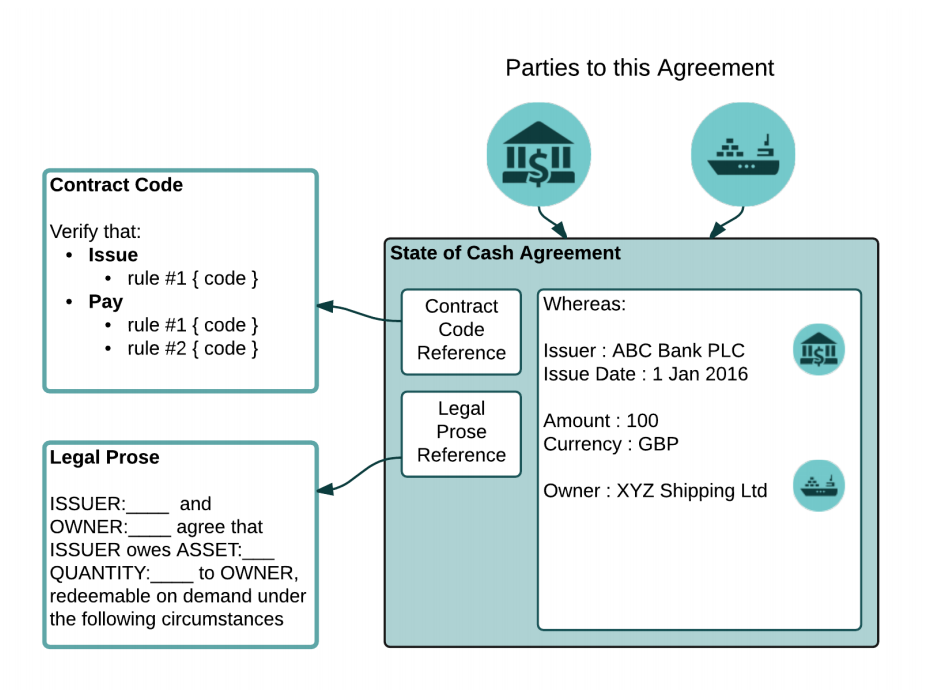
\includegraphics[scale = .4, center]{partiesto}
\caption{上图所示的状态对象,代表某个虚拟的航运公司在一家商业银行拥有一项100英镑的现金索赔权。状态对象通过哈稀算法记录其对应的法律文件和合约代码之间的显性关联关系,同时通过合约代码控制其转换。}
\end{figure}

与其他系统相比,我们专注于协议状态,而其他系统中参与方必须达成共识的数据是整个账本的状态或整个虚拟机的状态。Corda平台提供三种主要工具来达成全局分布式共识:
\begin{itemize}
  \item  智能合约逻辑,根据预先约定的规则,确保状态转化的有效性;
   \item  唯一的时间戳服务,以消除冲突同时保证事务顺序性;
  \item   一个业务流程处理框架,以简化多个参与方之间复杂多步骤协定的编写过程。
    \end{itemize}
    
\subsection{共识机制}
在Corda平台中,记录的更新要通过”交易“,交易会覆盖已有的状态对象,生成新的状态对象。共识机制可分为两个方面:
\begin{enumerate}
\item 交易有效性:参与方通过检查相关合约代码成功运行并持有全部必需的数字签名,便可以确认预期更新的可定义输出状态的交易是有效的,并且任何与之相关的交易都是有效的;
\item 交易唯一性:参与方如果确认该交易是所有输入状态的唯一使用者,即可确认其唯一性。也就是说,没有其他交易可以推翻我们之前达成的共识(有效性和唯一性),使用同一状态。
\end{enumerate}

参与方通过独立运行相同的合约代码并验证其逻辑性,便可对交易有效性达成一致。然而,就交易唯一性达成共识,需要一个预先选定的观察者,很多情况下要求观察者具备独立性。

\begin{figure}[H]
    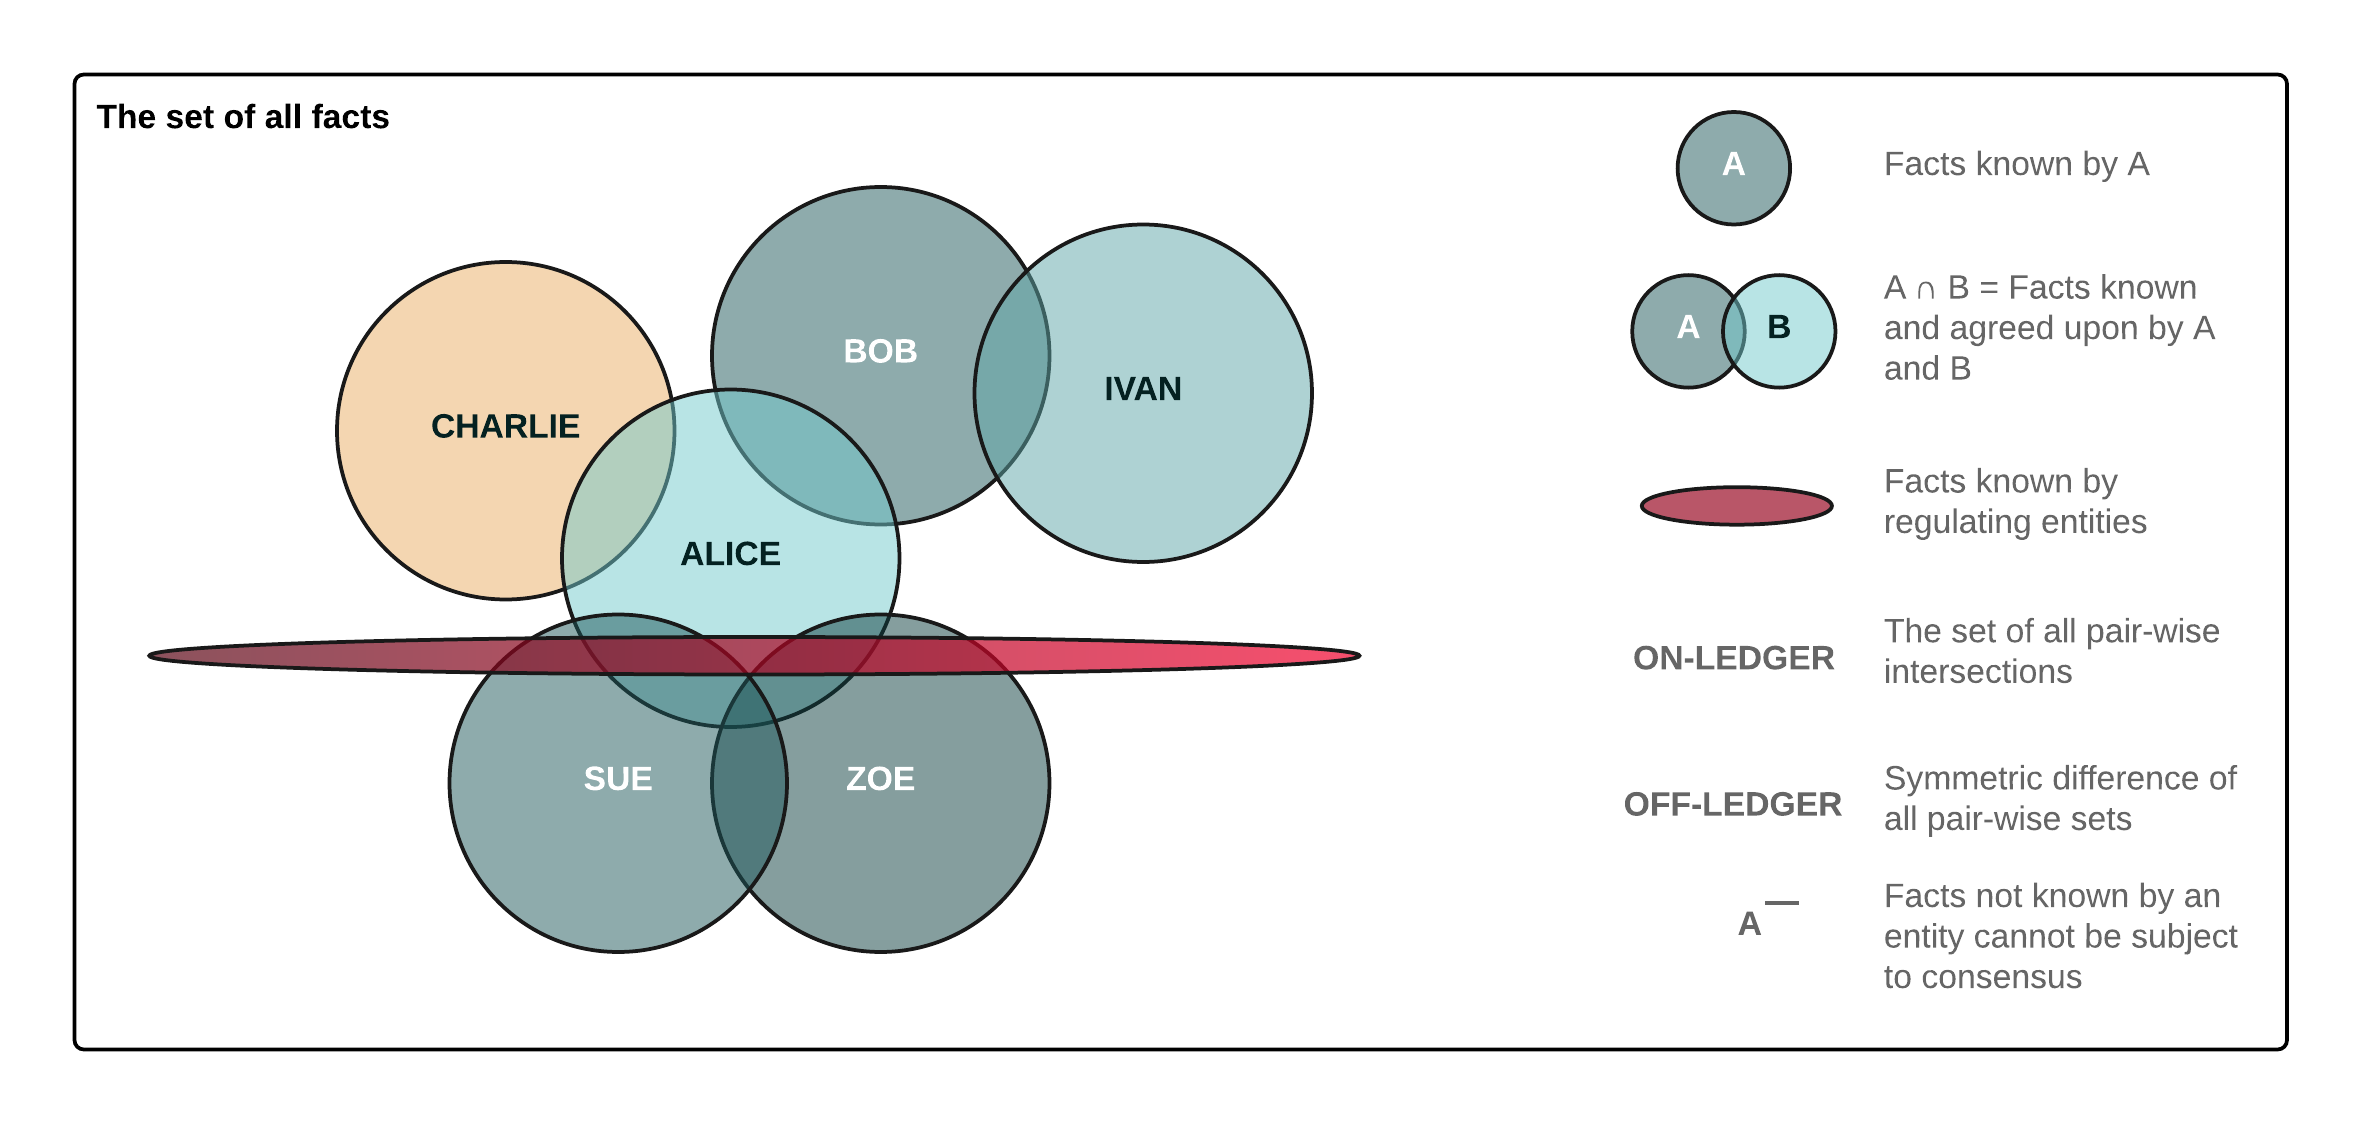
\includegraphics[scale = .5, center]{Consensus}
    \caption{上图所示,仅该交易参与方才能就交易有效性达成共识。因此,数据仅对需要查看的参与方共享。而其他平台一般在账本层面达成共识。所以, Corda系统中的任何角色,都只能看到整个系统管理的全部数据的子集。如果系统中至少两个角色就一份数据是否存在和细节问题达成共识,我们就称其为“账本上的数据”,系统允许任意组合的角色参与到所有指定数据的共识建立进程中。仅被唯一角色拥有的数据,被称作为“账本之外的数据”。}
\end{figure}

Corda提供”可插拔“的唯一性服务,旨在提高隐私性、扩展性、法律系统兼容性和算法的敏捷性。单一服务可能由众多相互不信任的节点组成,这些节点通过一种拜占庭容错算法组合在一起,或可能非常简单,像一台单独的机器。在某些情况下,例如状态的变化需要全部相关参与方签名,这时候可以不需要唯一性服务。 

需要重点指出的是,这些唯一性服务仅用于证明某个状态的变化是否是因为某个特定交易的发生引起的;它们不需要证明交易本身的有效性,那是交易参与方的责任。这意味着,唯一性服务不需要访问任何交易的完整数据,与其他分布式账本和区块链设计方案相比,大大提高了系统的隐私性和扩展性。这项设计决策,是在共享账本框架中做出权衡的重要抉择,我们即将发布的技术白皮书会对其作更详细的说明。

\subsection{商业逻辑}
Corda平台通过智能合约代码执行商业逻辑,由一段纯函数构成,只用来接受或者拒绝一次交易,可能是由更简单和可复用的函数组成。这些函数将交易解释为,通过应用(智能合约)命令来使用输入状态并生成输出状态,如果预期操作有效,则接受该项交易。合约定义了账本的部分商业逻辑,而且具有灵活性:某些配置里各个节点将会在沙箱内下载并运行合约,并不需要审查,尽管我们的设想是监管环境下的Corda平台配置将使用签名代码。 

我们选择Java虚拟机来执行合约及验证有效性,因为Java虚拟机有多个已有库和丰富的技术积累,并且利用已有产业标准,便于银行重复利用现有合同内代码。不过,我们给Java虚拟机增加了一个定制沙箱,比普通的JVM沙箱严格得多,不仅执行安全需求,还支持确定性执行。跟以太坊一样,选择标准化字节码集Bytecode集而不是某一门编程语言,可允许用户在合约语言设计方面进行创新,或根据自身喜好复用已有编程语言。这也便于用户直接使用内部程序的合约代码,一旦合约通过审查便可使用,这将大大简化应用开发过程。

\subsection{核心金融概念}
Corda的基础架构深受三个架构领域影响深远的用例影响,被视为具有代表性的共同问题,也可能是有所针对性的。这三个用例包括:现金,证券托管和衍生品合约。在所有三个用例中,我们设想它们为金融协议的案例:
\begin{itemize}
\item 现金余额(例如:“我与以下银行达成一致,银行欠我一百万美元”)
\item 证券托管(例如:“我与以下托管银行达成一致,我拥有以下公司的1000股股票”)
\item 双边衍生品协议(例如:“银行A和B同意他们是以下利率互换协议(IRS)的参与方,这意味着他们在预定时间根据协商一致的清算公式对以下现金流进行互换”)
\end{itemize}
就这些例子中的一个而言,Corda的现金设计对商业现实进行了明确建模,“储存在银行中的钱”的概念不复存在,只有所有者对一家指定机构的现金索取权的概念。所以,我们的核心现金合约极其简单却不失强大:我们记录现金发行者的法律身份、货币种类、现金数目、现金所有者(其他信息比如索取权的性质,明确指定管理此协议的法律条文,法律条文也会说明发生争端后的解决流程),在这些基础上建立其他所有与现金相关的概念(支付、结算和其他)。
\begin{figure}[H]
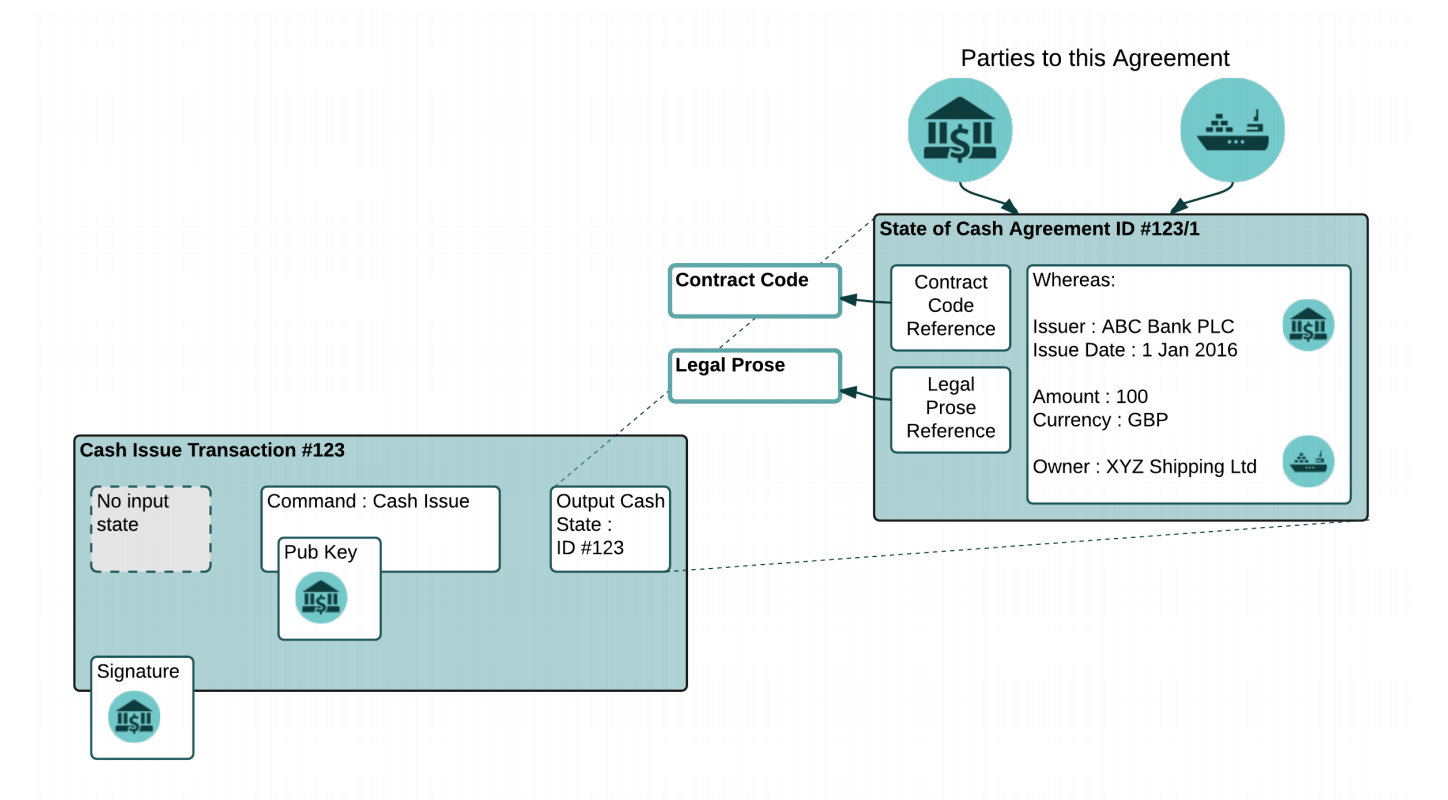
\includegraphics[scale = .4, center]{cash}
上图展示了一种最简单的Corda平台交易:发行交易。我们发现生成一个新的现金状态,由一家商业银行发行给一家虚构的航运公司。该发行交易由发行银行签名。从这个简单模型,可以构建出更复杂的交易,例如支付、货银对付合约和期债。
\end{figure}
Corda模型总结
我们模型的核心概念是:
\begin{itemize}
\item 状态对象:代表两个及以上参与方之间的协议,由机器可读的合约代码控制。合约代码引用并旨在执行人类可读的法律条文。交易:通过生命周期转化状态对象。
\item 交易协定或商业工作流:在无中心控制的情况下让参与方可协调操作。
\end{itemize}

有选择性地严格限制可用的编程技术,让决定权最大化,但是可共享的状态数量必须最小化。

状态对象(数据)的组合、合约代码(允许性操作)、交易协定(商业逻辑编排)、任何必要的API、钱包插件、UI组件,都可以被认为是一个共享的账本应用程序,或Corda分布式应用程序(CorDapp)。这是一个核心的组件集,是平台上任何一个合约开发者都期待去创建的。 

%\begin{figure}[H!]
%\includegraphics[scale = .4, center]{image4}
%\caption{现在关于Corda平台生态系统内应用程序的观点}
%\label{fig:figure4}
%\end{figure}

%\begin{figure}[H!]
%\includegraphics[scale = .25, center]{image5}
%\caption{Another visual representation on how Corda will interact with the financial ecosystem.}
%\label{fig:figure5}
%\end{figure}

\section{Corda平台与其他平台的对比}
Corda平台的创建得益于我们与金融从业者的广泛合作,设计更是始终围绕着他们的需求。当然,Corda设计灵感也来自于以往的成果,包括Todd Boyle和Ian Grigg在论文中关于三式簿记的介绍\cite{Triple},以及已有分布式账本平台(例如比特\cite{Bitcoin}币和以太坊)的相关因素。因此这也便于不了解Corda的人借助这些平台来更好地理解Corda。 
\subsection{与比特币的对比}
Corda与比特币有以下几个显著相似点: 
\begin{itemize}
\item  通过交易创建和使用的状态不可变的,这是一样的;
\item 交易有多项输入和输出。比特币有时会用“未使用的交易输出集”(UTXO集)指代账本作为结果输出;
\item 合约是纯函数;合约并无存储功能,也不能与任何其他事物进行交互。对于同一项交易,合约的“验证”函数永远输出相同结果。
\end{itemize}

然而,比特币交易有单一且严格的数据格式,而且除了比特币数量和相关使用规则(脚本),只能保存极少的数据。曾有人试图打破这种限制:通过在合约代码的半标准化处嵌入数据,以便可以通过模式匹配来提取数据,但这种方法并不有效。相比之下,Corda平台内的状态可以包含任意类型的数据。另外,Corda平台上的交易不仅可以调用输入合约,也可以调用输出合约。比特币交易的确认机制仅由已使用输入状态的合约代码控制。而Corda的“合约”概念,指的是可以处理各种任务的一系列商业逻辑,而不限于交易验证。比如,现在Corda上的合约还包含生成有效交易的代码(一般在比特币中被称作“钱包代码”)。

比特币脚本只能获取一串固定的字节数组作为输入项。这意味着合约无法判断整个交易的结构,对合约的功能造成了极大限制。而我们的合约是图灵完整的,可使用任何普通编程语言在JVM上工作。	
Corda允许在交易中指定任意精确的时间边界,而不依赖挖矿产生区块的时间。这至关重要,我们设想的许多合约类型也支持必要精准时间,同时也因为我们主要的共识机制执行方案是使用区块自由的冲突解决算法。这里需要强调的是,Corda并未使用工作量证明机制(POW),也没有“挖矿”的概念。

\subsection{与以太坊的对比}
和以太坊相似,Corda平台上的代码运行在相对强大的虚拟机上,并能包含复杂的逻辑。可用非汇编程序设计语言编写合约程序。二者都旨在为不同类型的金融合约建模。

然而,以太坊中的“合约”是指程序的实例化,每个参与节点都对其进行复制和维护。这种实例化非常像面向对象编程中的对象:可以接收和发送消息,更新本地存储等等。相比之下,我们对智能合约的执行方法用代码表示是一组函数,其中仅有一个函数用来保持系统同步(验证函数)。该函数是纯函数而且无状态(比如,它不可能与系统的其他部分进行交互)	。因为合约没有任何类型的可变存储器,因此没有“消息”的概念。以太坊宣称自己是不限于金融逻辑的平台,理论上可以应用于各行各业。而我们的Corda平台暂不考虑非金融应用,至少前期如此。

%\section{实例:现金}
%状态对象代表了参与方之间的一项协议。

%状态包含任意数据,也包含了至少一个对一段合约代码哈希算法的引用(以字节码表示、在虚拟机内沙箱运行的程序),以及一个对一段法律条文哈希算法的引用(以司法系统或其他争端解决体制认可的方式提供法律语境)。合约代码(本文其他部分也用”合约“指代)是全局共享的商业逻辑。合约永远定义一个验证函数,该函数为纯函数,无论哪一方调用,都可确定状态的转换是否有效。验证函数不会核对交易是否符合任何一方的利益,只会强制执行约束,各个节点必须自己确定交易是否符合己方的利益。这一点后面会继续说明。

%上图展示了一个现金状态对象,代表了对100美元的所有权。此对象引用了对其有约束力的合约以及相关的法律条文。因为这是一项现金合约,法律条文文件会说明一方向另一方发行的现金债务的条款与条件:什么情况下现金对象可换成传统银行账户内的现金余额,或者换成向其它账户的电子汇款?若产生争议将如何解决?诸如此类。另外,法律条文还会规定这项各方同意由计算机代码自动执行的合约的权利、义务和条件。法律条文域直接委托到代码域。

%而且很重要的是,有几点信息法律条文不会说明:发行者是谁?用哪种货币?状态对象会包含这些信息(此例中发行者是巴克莱银行,货币是美元)。法律条文、合约代码、状态对象获取的参数再加上相关的数字签名共同定义了参与方之间的协议。

%接下来,我们描述了一个如上图的状态对象如何使用Corda架构的其他组件来经历演变、处理、在参与方之间转移。

%请注意:层级非常高的时候,Corda的设计与比特币的”UTXO模型“很相似,但是也有一些非常显著的区别。我们选择UTXO风格的模型,而不是以太坊使用的账户/余额模型,是经过了深思熟虑的决定,本平台的隐私性和扩展性正建立在此基础之上。

\section{路线图}
为了达成这项设计方案,我们首先用代码模拟并绘制了Corda组件的产品原型图,以验证设计概念的方方面面。Corda模型有望在中短期内交付,以下是Corda模型的部分(并非全部)扩展方向。
\begin{itemize}	
 \item 交易分解与强化唯一性服务:整合多种机制以有选择地隐藏部分交易,包括唯一性服务的模糊处理;
\item 合约验证沙箱:显式链接最小的Java库白名单;
\item 基于插件的钱包,用于位置推理;
\item 数据库或网关对应所属(或其他)商业逻辑执行者(比如中央机构或估值代理方),参与方在账本上可验证执行者身份。
\item 使用Corda模型来管理用户身份;
\item 互操作性和数据集成:尤其参照FpML和ISO20022,支持其他数据格式和其他平台的集成或互操作性;
\item 为涉及的数据构建应用程序;
\item 使用技术来强化隐私性,比如不规则分布地址、零知识证明和资产发行方案等;
\item 未来金融工具的参考合约;
\item 原生支持资产组合层级的商业逻辑,比如状态对象的聚合。
\end{itemize}
\section{结论}
相比现有的分布式账本和区块链平台,Corda平台的创建有着明确的目的,即记录和执行注册金融机构的业务协议,而并非为所有问题提供解决方案。因此,Corda的数据分配和交易语义均独辟蹊径,但仍保持了分布式账本的特性,金融机构也正是因为这类特性才对R3之类项目产生兴趣,换而言之,就是采取一种自动化且可实施的方式来确保金融协议的可靠执行。
\bibliographystyle{unsrt}
\bibliography{Ref}
\end{document}
